\chapter{Overview e progettazione di sistema}
\label{chap:overview e progettazione di sistema}
In questo capitolo viene messo in luce lo scopo dell'elaborato realizzato con particolare attenzione alle scelte progettuali adottate e alle ricerche effettuate per implementare l'argomento trattato, onde presentare un quadro generale completo. Viene, inoltre, descritta l'architettura del software, sottolineando ed approfondendo le sue principali componenti.

\section{Scopo del progetto}
\label{sec:scopo del progetto}
Lo scopo principale del lavoro di tesi è quello di creare un sistema distribuito che permetta la visualizzazione real time, la storicizzazione e l'analisi delle transazioni  provenienti dalla blockchain di bitcoin. L'obiettivo, dunque, è quello di riuscire a creare un sistema che gestisca grandi quantità di dati in un ambiente distribuito, garantendo affidabilità e consistenza dei dati anche in caso di guasti.
\\Il sistema si rivolge ad un pubblico che vuole fare analisi delle transazioni processate dalla rete bitcoin. L'utente infatti, può controllare in real time le ultime transazioni elaborate, monitorare l'intera rete blockchain per risalire a tutta la catena di transazioni, oppure controllare gli hash (indirizzi) che hanno avuto maggior punteggio di PageRank.
\\Le ultime transazioni elaborate, hanno una serie di informazioni di dettaglio come il blocco di appartenenza, l'hash che ha generato quella transazione, il timestamp ed i destinatari dei bitcoin. Mentre per quanto riguarda il monitoraggiio dell'intera blockchain, l'utente può navigare con l'utilizzo del proprio mouse, in un grafo orientato rappresentante la storia di tutte le transazioni. Inoltre, il fruitore può controllare i nodi con il maggior punteggio di PageRank e localizzarlo all'interno del grafo.  

\section{Architettura  del progetto}
\label{sec:architettura del progetto}
Le principali scelte di progetto sono state prese coerentemente con lo stato dell’arte e si è tentato di non introdurre nuova complessità al panorama esistente, ricorrendo a tecnologie, protocolli e standard già esistenti ed affermati, senza definirne di nuovi. Quindi, l’architettura dovrà essere sufficientemente generale in modo da poter garantire nuovi sviluppi ed evoluzioni future e da non comportare l’esclusione a priori di determinate soluzioni e tecnologie. 
\\Il sistema, quindi, può essere diviso logicamente in due moduli:
\begin{itemize}
	\item \textbf{Il Sistema distribuito (back-end)}: E' la parte non visibile all'utente. Si occupa del recupero dei dati dalla blockchain di bitcoin, della storicizzazione e della pubblicazione sui topic di kafka. Interamente scritto in Java, comprende Bitcoind, Spark, Hadoop, Neo4j, Zookeeper.
	\item \textbf{Webapp (front-end)}: E' la parte visibile all'utente finale. Si occupa della rappresentazione grafica delle transazioni. Scritto in principalmente in Javascript, utilizza la potenza di NodeJS per creare l'interfaccia grafica. Integra nel proprio ecosistema Express Handlebars, WebSocket, MaterialCSS e D3js.
\end{itemize} 

\begin{figure}[H]
	\centering
	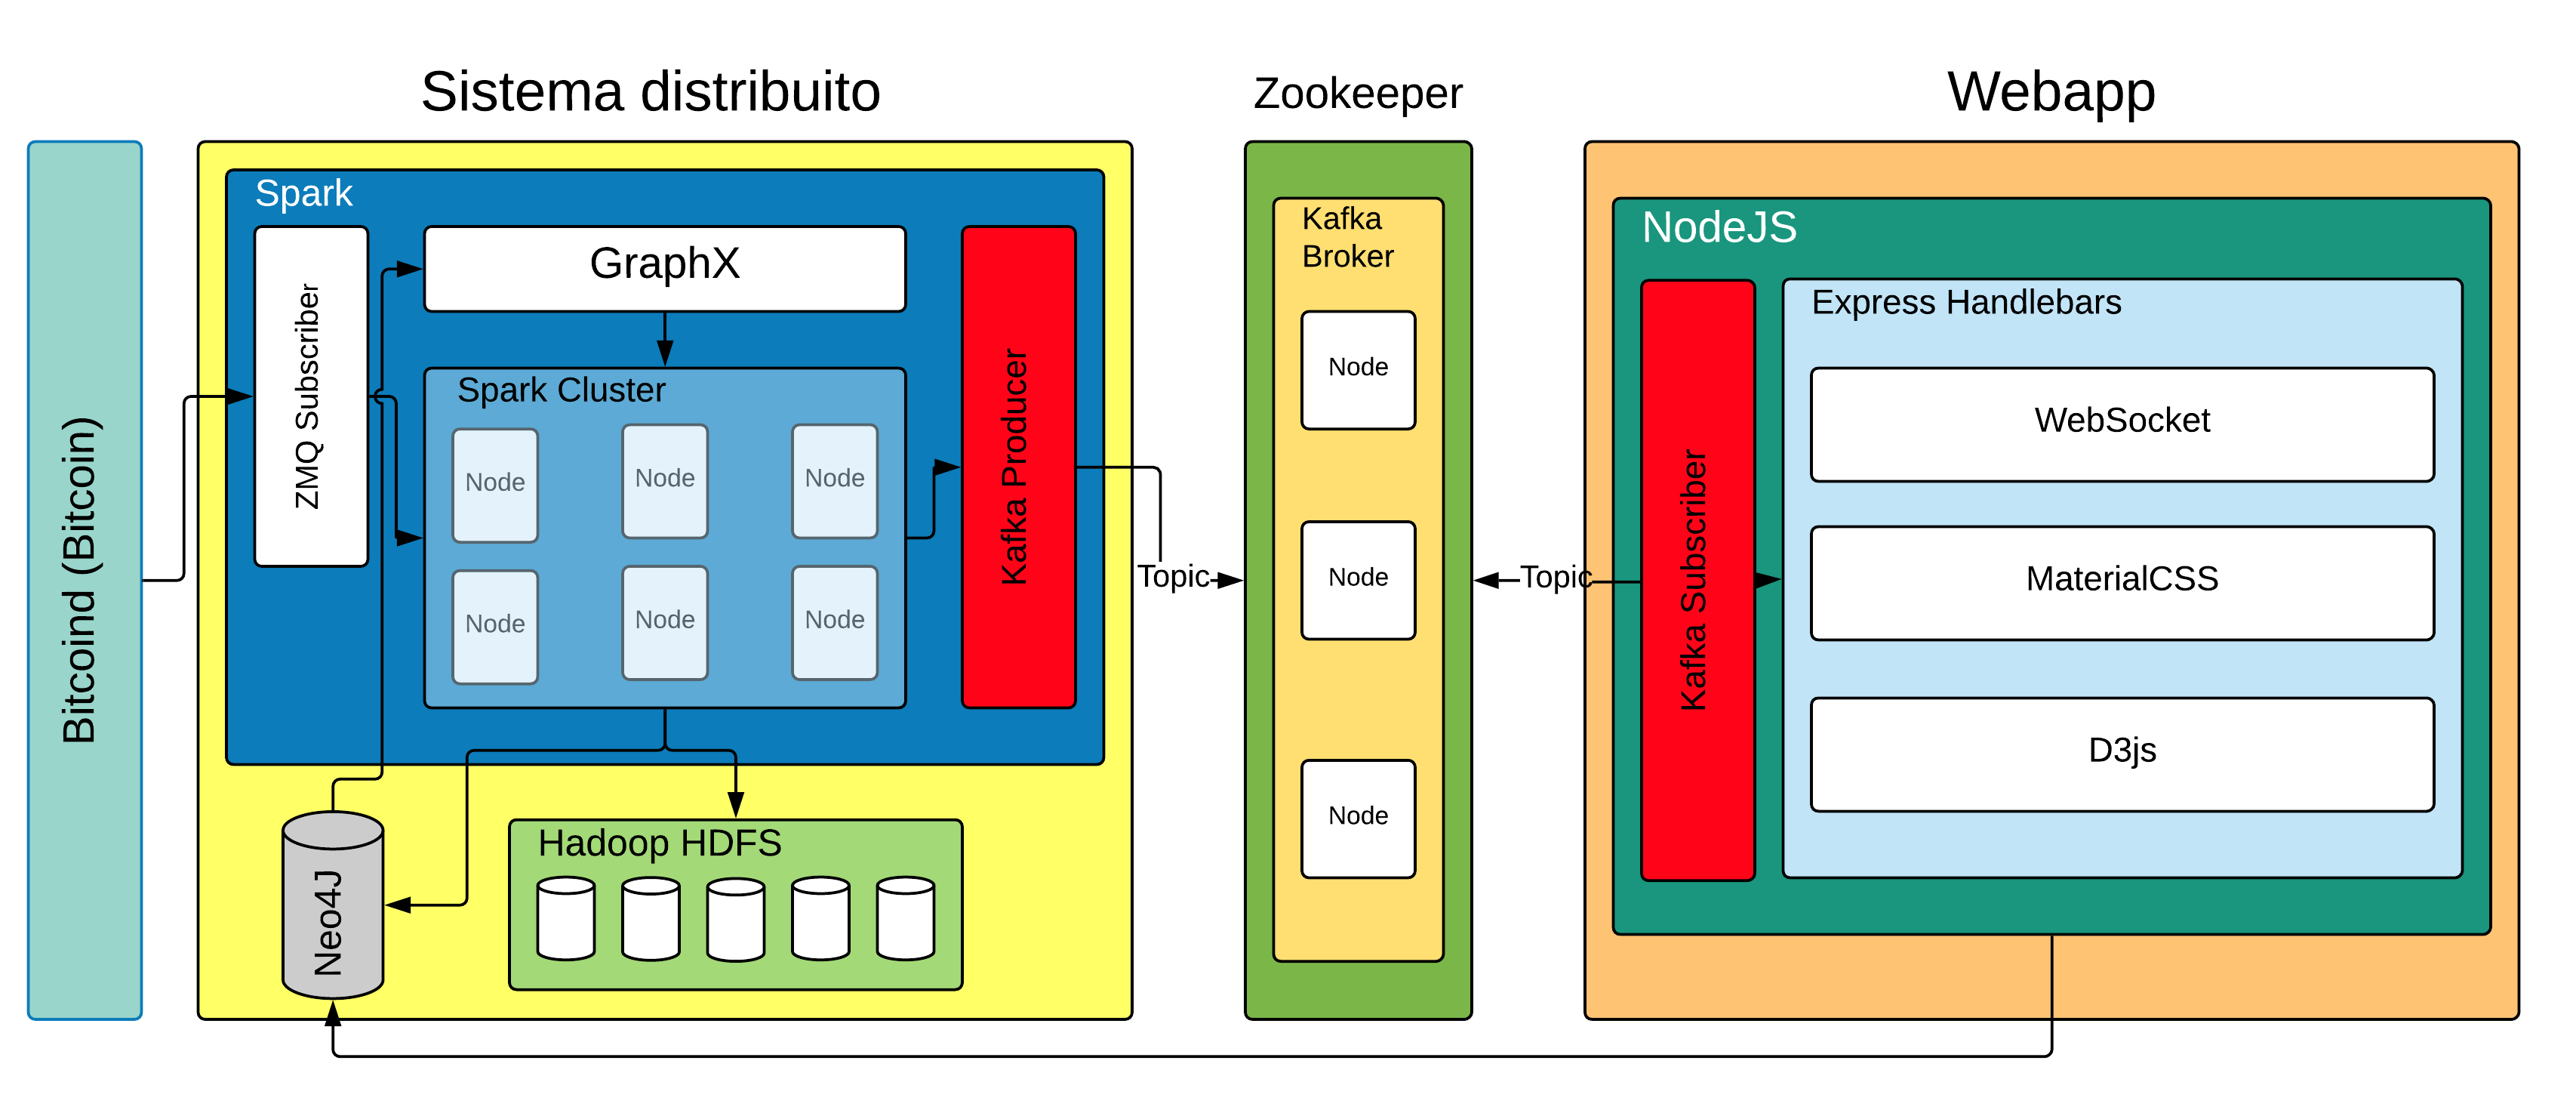
\includegraphics[width=\textwidth]{images/architetturaTesi.png}
	\caption{Architettura completa.}
	\label{fig:softwareArchitetture}
\end{figure}

La prima grande sfida, quindi è stata quella di trovare un framework o un tool che permettesse di programmare su di un sistema distribuito, senza complicarci la vita. Facendo ricerche sul web la tecnologia che più si accostava meglio al mio problema è stata Apache Spark [\ref{sec:spark}]. Questo strumento riesce a garantire a pieno i vincoli che ci siamo imposti. Risolto il problema infrastrutturale si è proceduto all'analisi dei singoli sottoproblemi. 
\\L'applicazione fa uso dei blocchi grezzi da bitcoin, per testare il carico di lavoro sul sistema, provenienti dal software nativo del progetto Bitcoin: Bitcoind [\ref{sec:bitcoind}]. Bitcoind è un demone che invia blocchi o transazioni (a seconda di come lo si imposta) su di una coda di tipo publisher-subscriber tramite protocollo ZeroMQ [\ref{sec:ZMQ}]. I dati, quindi, sono prelevati da Bitcoind grazie all'implementazione di un subscriber creato ad hoc.
\\Ottenuti i blocchi dalla coda, il problema si è spostato sul conservare i dati ottenuti in modo da poterli processare ed analizzare. Fortunatamente, Spark offre una nativa collaborazione con il FileSystem distribuito Hadoop [\ref{sec:hadoop HDFS}], permettendomi di tenerli salvati su una memoria di massa distribuita.
\\Oltre ad Hadoop, i dati sono stati immagazzinati in Neo4j [\ref{sec:neo4j}]. Un database NoSQL che permette il salvataggio dei dati sottoforma di grafo, cosi da poter gestire facilmente i collegamenti tra le varie transazioni.
\\L'ultimo step, è stato quello di fare analisi delle transazioni, trovando i nodi con il maggior PageRank [\ref{sec:graphx (PageRank)}]. Anche in questo caso Spark è venuto in contro grazie al modulo GraphX, contenuto nel framework, il quale contiene algoritmi (come il PageRank) già sviluppati per l'analisi sui grafi.
\begin{figure}[H]
	\centering
	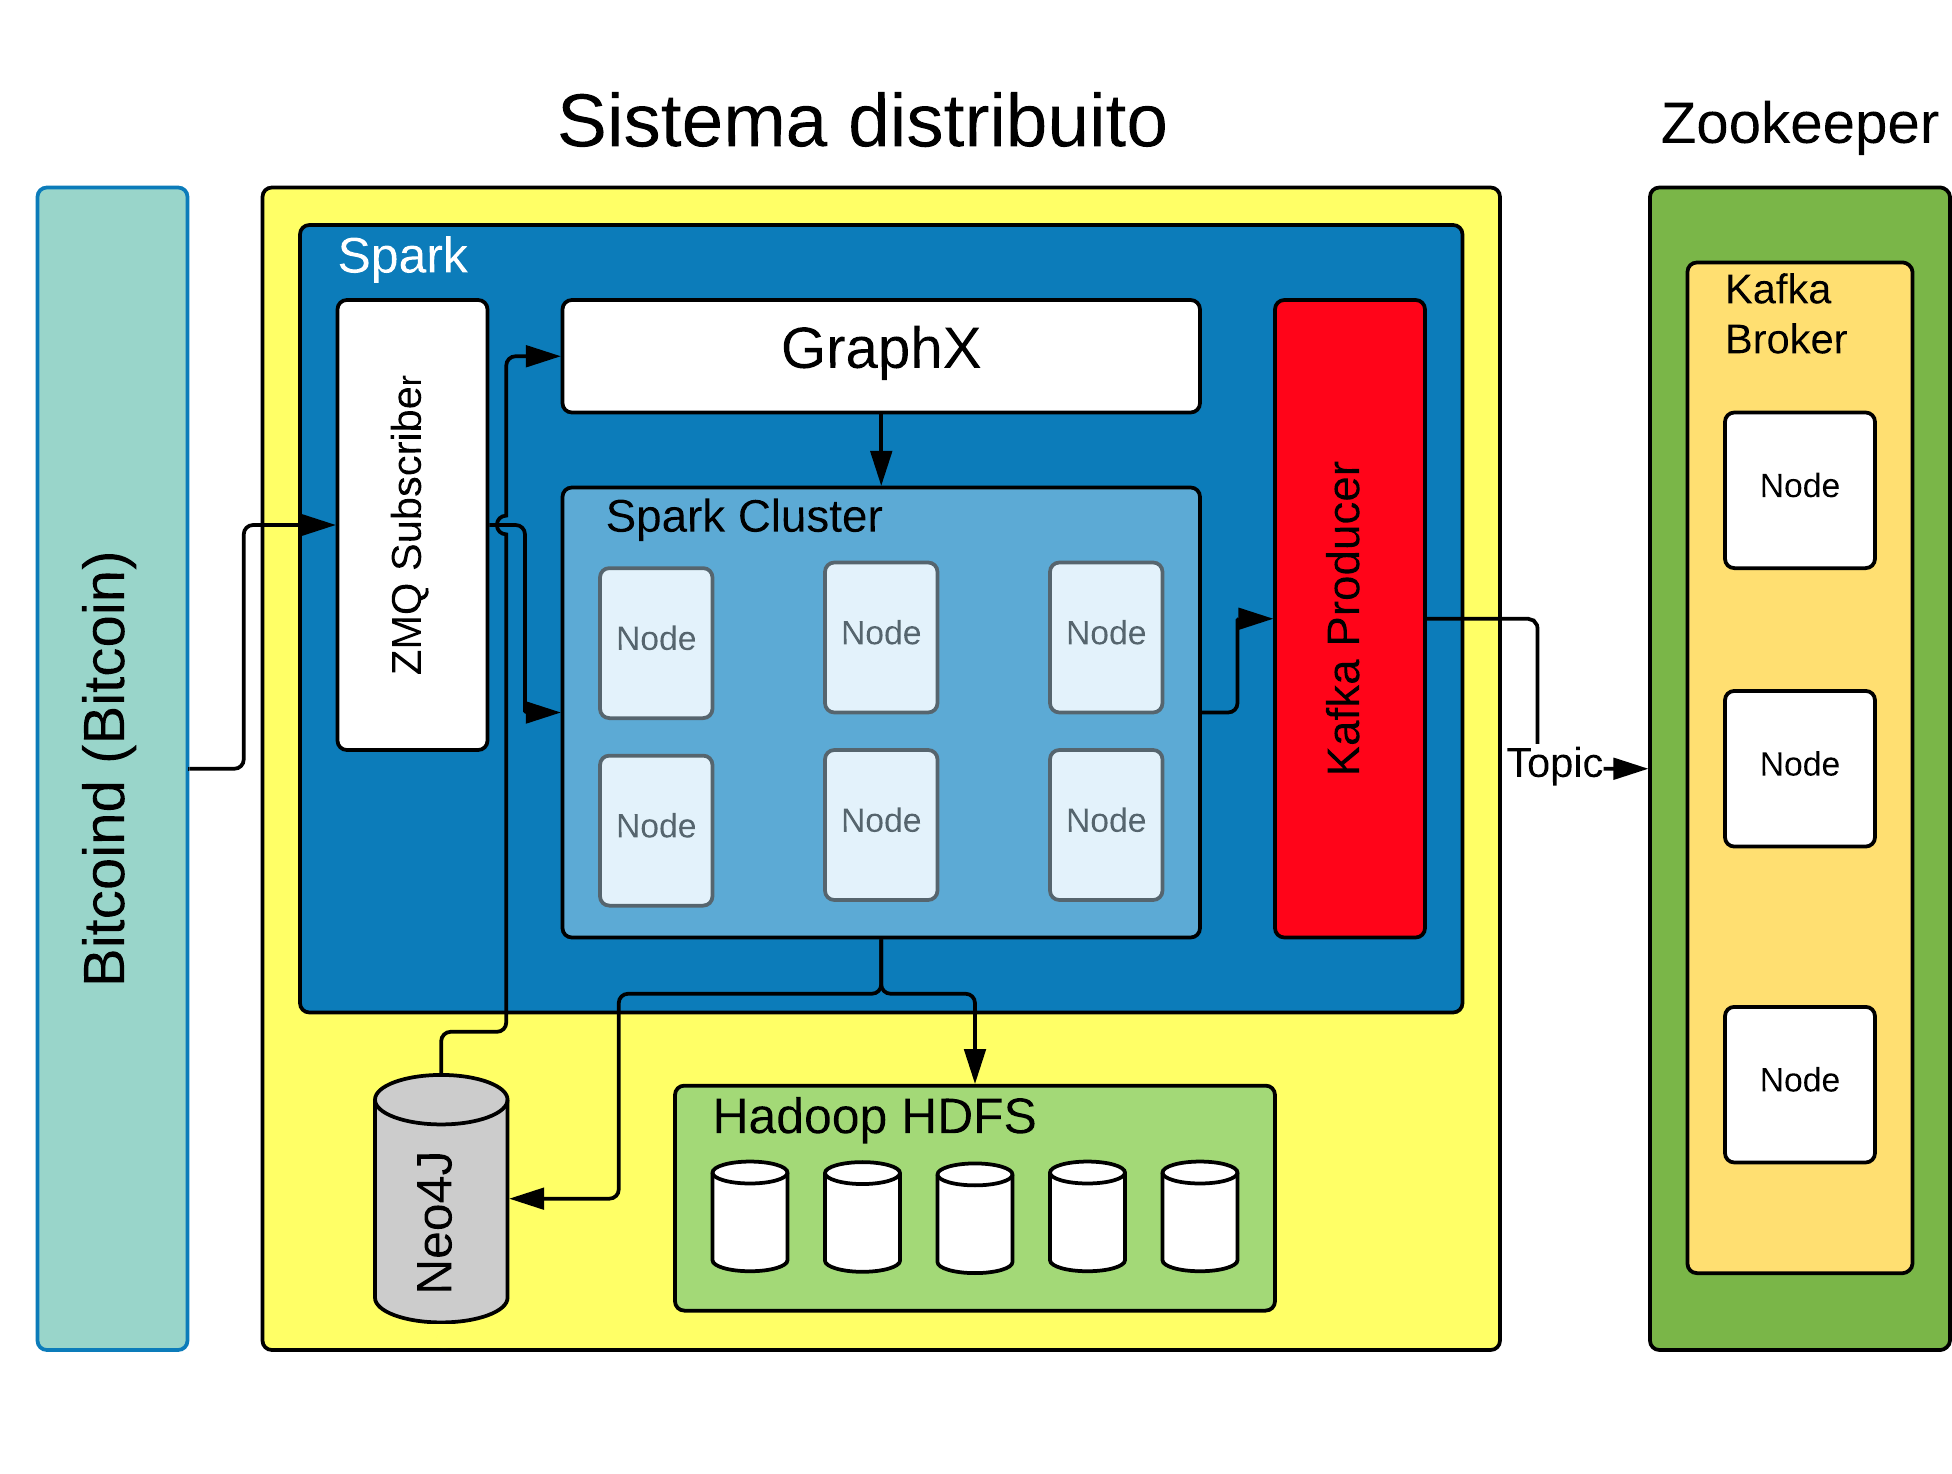
\includegraphics[width=\textwidth]{images/sistemaDistribuito.png}
	\caption{Architettura in dettaglio del sistema distribuito.}
	\label{fig:distribuitedSystemArchitetture}
\end{figure}  
Una volta che il sistema distribuito è completo, non resta che mostrare i risultati ottenuti. Le scelte nel campo del front-end sono migliaia ma per semplicità ed una forte attitudine ai sistemi real-time si è preferito usare NodeJS [\ref{sec:nodejs}]. NodeJS ha dei moduli che permettono l'accesso a Kafka, il tramite tra la parte di back-end e front-end. Inoltre, con NodeJS è stato creato un sito web, cosi da consentire agli utenti dal proprio browser, di visualizzare lo stato delle transazioni, i valori del PageRank e le transazioni che arrivano in real time.
\begin{figure}[H]
	\centering
	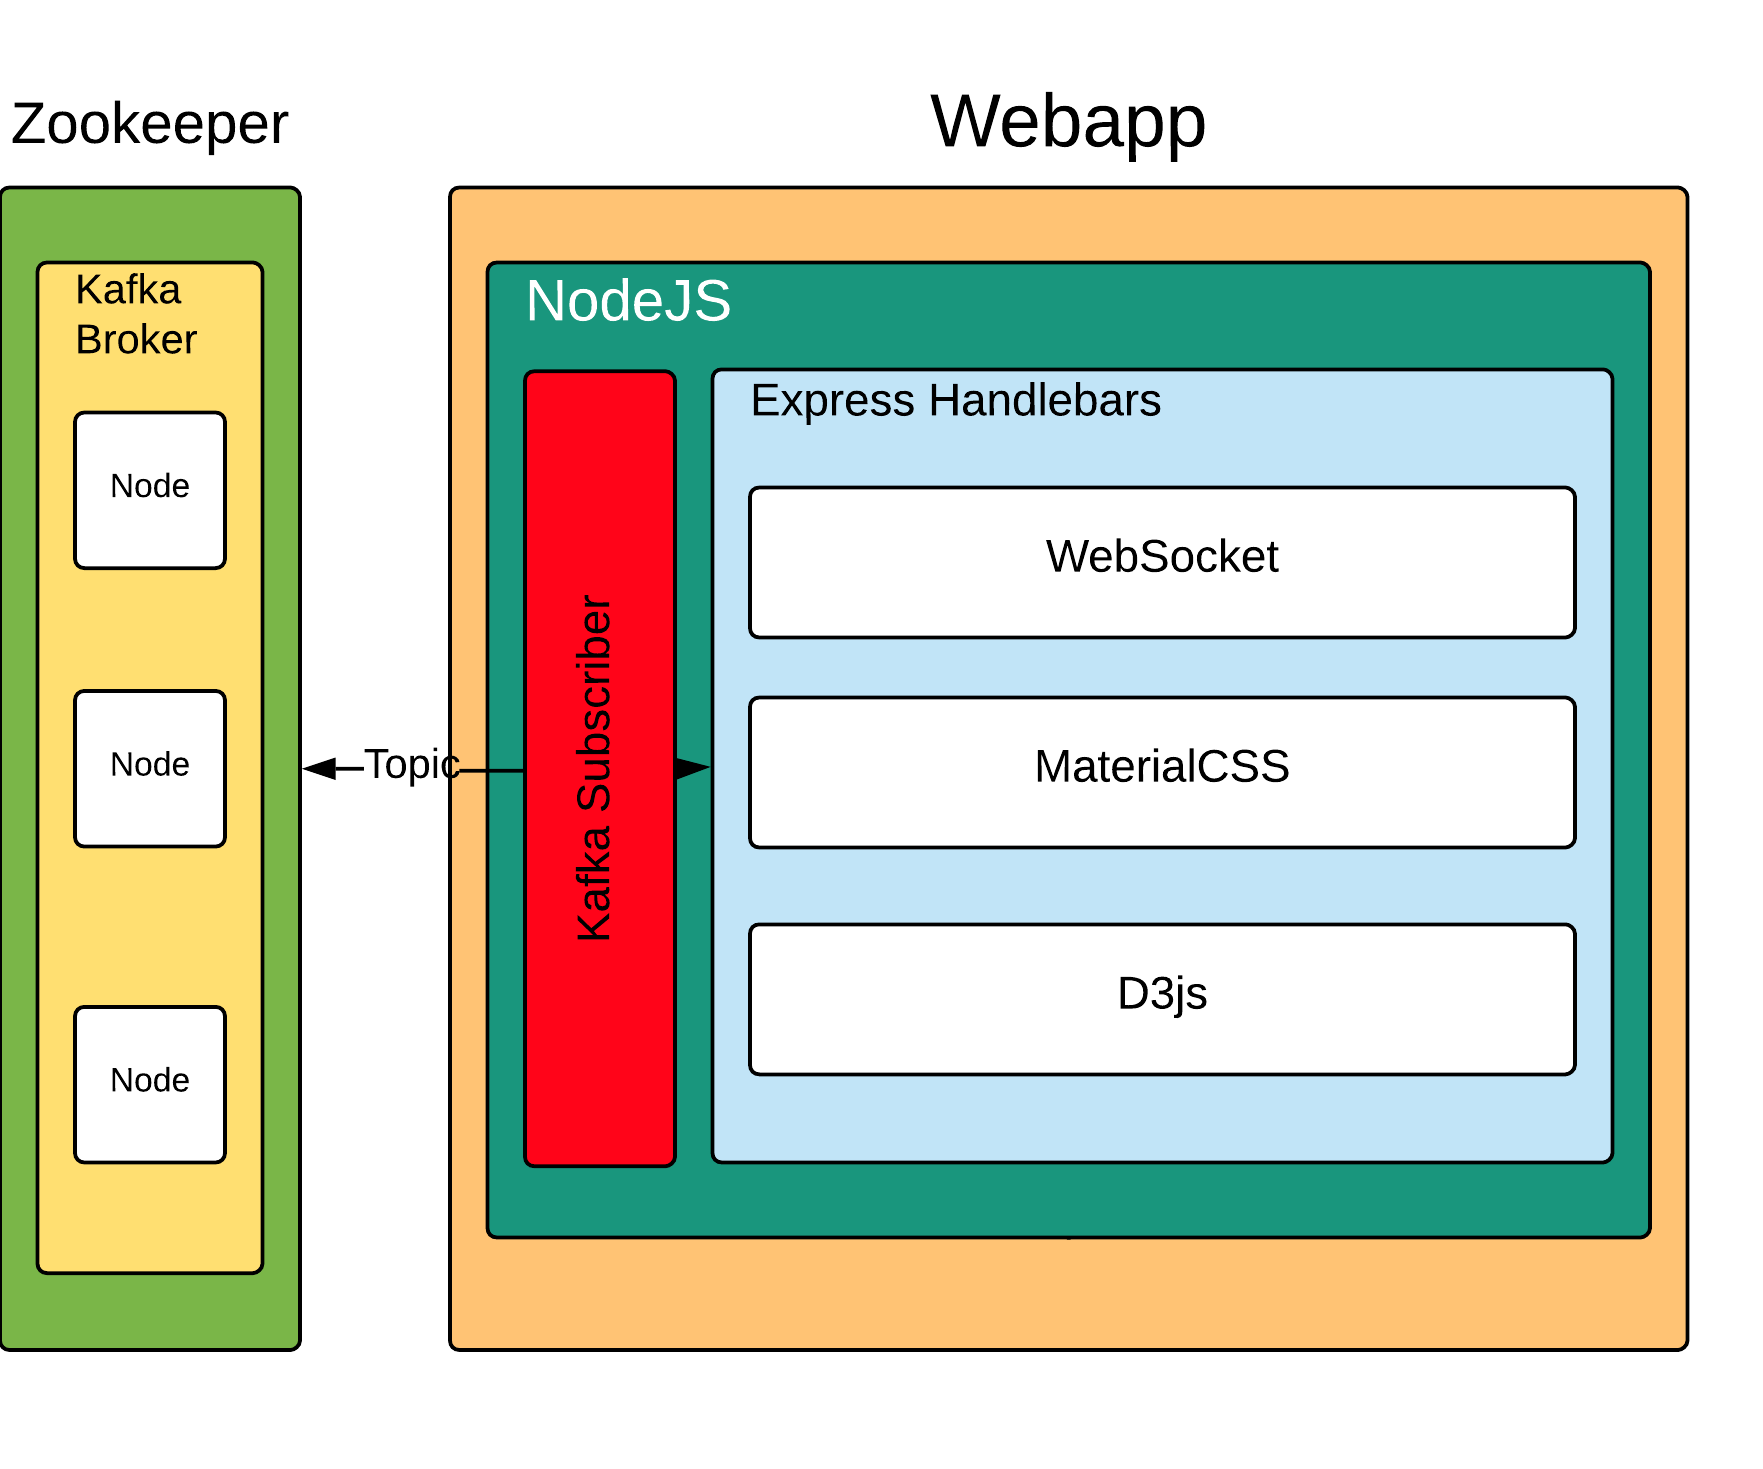
\includegraphics[width=\textwidth]{images/webApp.png}
	\caption{Architettura in dettaglio della webapp.}
	\label{fig:webAppArchitetture}
\end{figure}
\section{Sistema distribuito}
\label{sec:sistema distribuito}
\subsection{Bitcoind}
\label{sec:bitcoind}
Bitcoind è un software che implementa il protocollo Bitcoin per l'utilizzo delle remote procedure call(RPC). Esso è anche il secondo client Bitcoin nella storia del network.\cite{wiki:bitcoind}.
Questo programma è la fonte dei dati per l'applicazione, difatti invia i blocchi  


\subsubsection{ZMQ}
\label{sec:ZMQ}

\subsection{Apache Spark}
\label{sec:spark}
Apache Spark è un framework di calcolo del cluster per l'elaborazione di dati su larga scala, progettato e implementato nel 2010 da un gruppo di ricercatori dell’Università di Berkeley a San Francisco \cite{spark:hadoop}. Questo progetto nasce dall'esigenza di migliorare le prestazioni dei sistemi distribuiti “MapReduce”. Per questo si sviluppa il concetto di Resilient Distributed Dataset (RDD), che è la teoria alla base del sistema Spark. Un RDD rappresenta un set di dati che è suddiviso in partizioni (Una tabella chiave-valore suddivisa in tante sotto-tabelle o un file diviso in tanti segmenti). Un RDD ha la proprietà di essere immutabile, cioè una volta creato non può essere cambiato se non creandone un altro. La creazione di un RDD avviene a partire dai dati su disco (presi da HDFS) o da altre fonti di dati. Una volta creato, un RDD può restare in memoria oppure può essere materializzato su disco. Ogni RDD è descritto da un set completo di metadati che consentono la ricostruzione di una delle sue partizioni in caso di fault. Spark nasce come un sistema per creare e gestire job di analisi basati su trasformazioni di RDD. Dato che gli RDD nascono e vivono in memoria, l’esecuzione di lavori iterativi, o che trasformano più volte un set di dati, sono immensamente più rapide di una sequenza di MapReduce; questo perchè il disco non viene mai (o quasi mai) impiegato nell’elaborazione.
\\Come detto in precedenza, Spark non utilizza MapReduce come motore di esecuzione; invece, utilizza il proprio runtime distribuito (DAG) per l’esecuzione di jobs su un cluster. Quando viene invocata un’azione su un RDD, viene creato un “job”. Un Directed Acyclic Graph o DAG è un grafo aciclico in cui ogni nodo è una partizione di RDD e ogni vertice è una trasformazione. A differenza di MapReduce, il motore DAG di Spark può processare pipeline arbitrarie di operatori e tradurle in un unico “job” per l'utente.
\\Spark, infine, sta dimostrando di essere una buona piattaforma su cui costruire strumenti di analisi, infatti ha moduli per il Machine learning (MLlib), Elaborazione grafica (GraphX), Elaborazione di stream (Spark Streaming) ed SQL (Spark SQL) \cite{spark:hadoop}.
\begin{figure}[H]
	\centering
	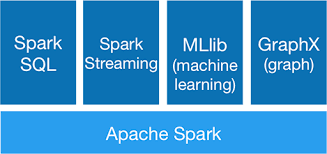
\includegraphics[width=\textwidth]{images/spark.png}
	\caption{Infrastruttura Spark.}
	\label{fig:sparkOverview}
\end{figure}
Nel sistema distribuito, poichè c'è l'esigenza di recuperare i dati in real time dalla coda di bitcoind, viene utilizzato Spark Streaming. Questo modulo è un'estensione dell'API Spark di base che consente l'elaborazione streaming, scalabile, ad alto throughput e con tolleranza agli errori dei flussi di dati in tempo reale. I dati, che possono provenire da diverse fonti, sono elaborati utilizzando algoritmi complessi espressi con funzioni di alto livello come \textit{map}, \textit{reduce}, \textit{join} e \textit{window}. I dati processati, infine possono essere inviati a filesystem (Hadoop) o database (Neo4j) per il salvataggio oppure ad altri moduli di Spark, dediti all'analisi, tipo machine learning (MLlib) o graph processing (GraphX). 
\\Internamente, Spark Streaming riceve streams di dati di input e li divide in batch, che vengono quindi elaborati dal motore Spark per generare il flusso finale di risultati. Per consentire il facile utilizzo di questi dati, fornisce un'astrazione di alto livello chiamata stream discretizzato o DStream, che rappresenta un flusso continuo di dati. E' possibile creare Dstreams da flussi di dati di input da sorgenti come Kafka, Flume e Kinesis o applicando operazioni di alto livello su altri Dstreams \cite{spark:home-streaming}. Internamente, un Dstream è rappresentato come una sequenza di RDD sulla quale possono essere effettuate le operazioni descritte in precedenza.
\begin{figure}[H]
	\centering
	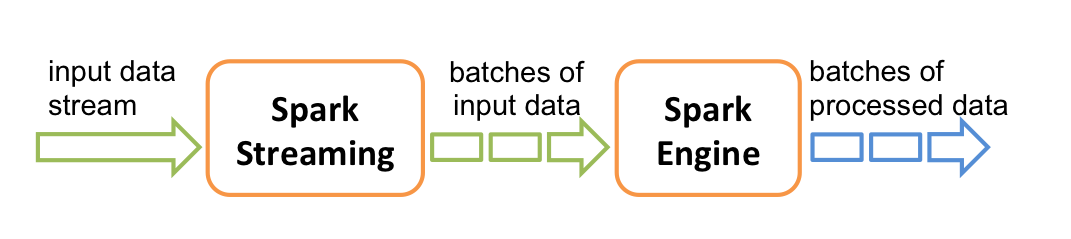
\includegraphics[width=\textwidth]{images/streamingSpark.png}
	\caption{Come vengono gestiti i dati in Spark Streaming.}
	\label{fig:streamingSpark}
\end{figure}
Nel sistema distribuito, per fare analisi dei dati provenienti dall'elaborazione di Spark, è stato scelto il modulo interno GraphX.
\\GraphX è un nuovo componetene di Apache Spark per grafi ed il calcolo parallelo (PageRank) su di essi. Estende gli RDD di spark introducendo gli Resilient Distribuited Property Graph, oggetti simili a grafi che permettono l'inserimento di proprietà per vertici e archi, rendendo facilitata l'implementazione. Inoltre, per aiutare nell'analisi, espone un insieme di operatori fondamentali (sottografo, joinVertices e aggregateMessages) come variante ottimizzata dell'API Pregel. In più, Graphx include una crescente collezione di algoritmi e costrutti per grafi per semplificare le attività di analisi \cite{spark:graphx}. Attualmente le sue API sono scritte in Scala, Java e Python.
\begin{figure}[H]
	\centering
	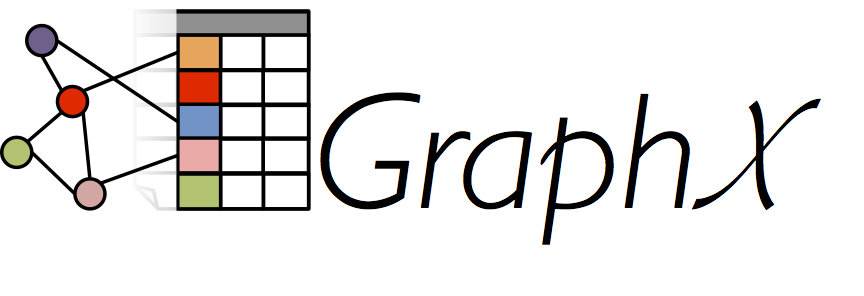
\includegraphics[width=\textwidth]{images/graphxLogo.png}
	\caption{Logo GraphX.}
	\label{fig:graphxLogo}
\end{figure}
GraphX, come detto in precedenza, gestisce i dati in memoria come se fossero grafi. Infatti, utilizza archi e vertici che hanno delle proprietà  connesse. Ogni vertice possiede un identificativo univoco a 64bit (VertexID), mentre, allo stesso modo, gli archi contengono gli identificativi di origine e partenza. Queste proprietà sono definite e tenuti in memoria come oggetti e di conseguenza con metodi creati ad-hoc per gestirli.  


\subsection{Hadoop HDFS}
\label{sec:hadoop HDFS}

\subsection{Neo4j}
\label{sec:neo4j}



\subsection{Zookeeper}
\label{sec:zookeeper}

\subsubsection{Kafka}
\label{sec:kafka}

\section{WebApp}
\label{sec:webapp}
Una applicazione web è una applicazione client/server per un ambiente stateless, cioè senza memoria, che utilizza le tecnologie internet. Con il termine Webapp si descrive un'applicazione accessibile via web per mezzo di una network, come ad esempio una Intranet o attraverso la rete Internet. Pertanto, saper programmare per il web significa conoscere i diversi meccanismi e strumenti per conservare o passare i dati, detti parametri, tra le diverse pagine dell'applicazione web. In pratica una Web-application, è un programma che non necessita di essere installato nel computer in quanto esso si rende disponibile su un server in rete e può essere fatto funzionare attraverso un normale Web browser (es. Google Chrome, Mozilla Firefox, Opera, ecc.). I client, dopo aver instaurato una connessione con il server, invia la richiesta per un servizio; il server dopo aver elaborato i dati necessari rende disponibile al client il servizio richiesto. A differenza dei siti web statici (HTML), l'applicazione web viene realizzata con una o più tecnologie (Javascript, Ajax, Servlet, Database ecc.) che permettono la creazione di un sito dinamico, cioè di un sito nel quale il contenuto delle pagine varia durante l'interazione.
\\Le applicazioni Web si pongono come valida alternativa alle tradizionali applicazioni Client/Server per vari motivi:
\begin{itemize}
\item \textit{Facilità di distribuzione e aggiornamento}: un'applicazione Web risiede interamente sul server, per cui la sua pubblicazione coincide con la distribuzione e l'aggiornamento ed è automaticamente disponibile a tutti gli utenti.
\item \textit{Accesso multi-piattaforma}: l'accesso all'applicazione è indipendente dall'hardware e dal sistema operativo utilizzato dagli utenti;
\item \textit{Riduzione del costo di gestione}: l'uso di Internet come infrastruttura per un'applicazione Web riduce notevolmente sia i costi di connettività che i costi di gestione dei client;
\item \textit{Scalabilità}: un'applicazione Web ben progettata può crescere insieme alle esigenze dell'azienda senza particolari problemi;
\end{itemize}
Per poter mostrare l'elaborazione di Spark nel sistema distribuito, si è preferito utilizzare una webapp per i motivi sopra citati. Questa applicazione web fa uso di tecnologie di ultima generazione quali NodeJs ed HTML5. Questo la rende fruibile a tutti gli utenti provvisti di Pc, Tablet o Smartphone con un browser installato. Nel seguente capito dunque vengono messi in luce i principali componenti che compongono la webapp, mostrando i punti forti di ogni tecnologia.
\begin{figure}[H]
	\centering
	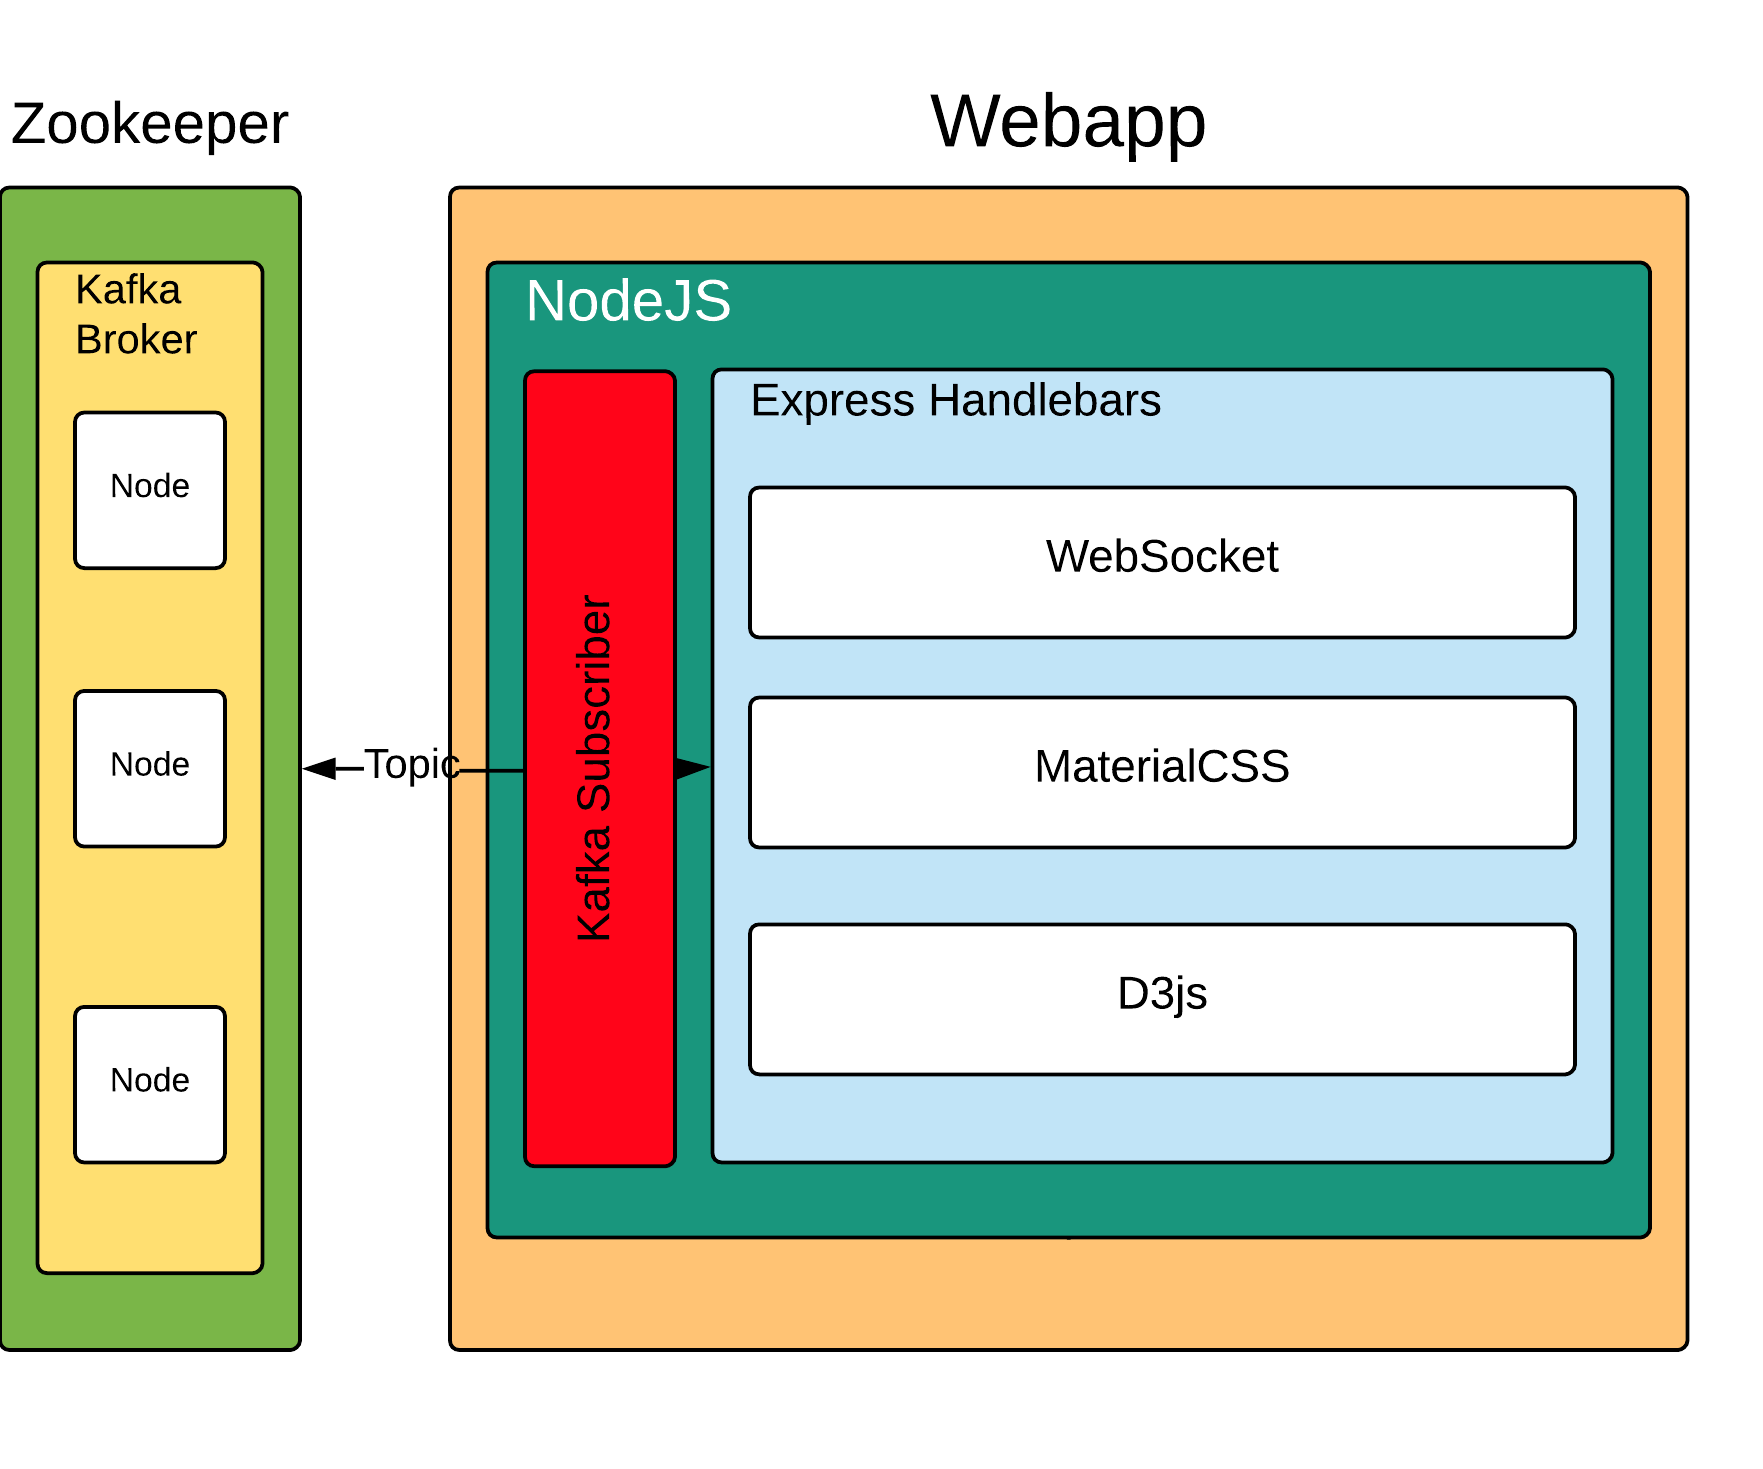
\includegraphics[width=\textwidth]{images/webApp.png}
	\caption{Architettura in dettaglio della webapp.}
	\label{fig:webAppArchitetture}
\end{figure}
\subsection{Node.js}
\label{sec:nodejs}
Node.js (anche conosciuto come Node o Nodejs) è un framework/piattaforma molto potente basato sul motore \textit{JavaScript V8} di Google Chrome, per creare facilmente applicazioni di Web veloci e scalabili. Pubblicata da Ryan Dahl nel 2009, viene utilizzato per sviluppare applicazioni Web intensive di I/O come siti di streaming video, applicazioni a pagina singola e altre applicazioni Web. Node.js è un ambiente open source, multi-piattaforma per lo sviluppo di applicazioni lato server completamente gratuito, utilizzato da migliaia di sviluppatori in tutto il mondo. Le applicazioni Node.js sono scritte in Javascript e possono essere eseguite all'interno del runtime di Node.js su OSX, Microsoft Windows e Linux. 
\\Utilizza un modello I/O non bloccante e basato sugli eventi che lo rende leggero ed efficiente, perfetto per applicazioni in tempo reale ad alta intensità di dati che funzionano su dispositivi distribuiti \cite{node:home}. Il modello di networking su cui si basa Node.js non è quello dei processi concorrenti, ma I/O event-driven: ciò vuol dire che Node richiede al sistema operativo di ricevere notifiche al verificarsi di determinati eventi, e rimane quindi in sleep fino alla notifica stessa. Solo in tale momento torna attivo per eseguire le istruzioni previste nella funzione di \textit{callback}, così chiamata perché da eseguire una volta ricevuta la notifica, che il risultato dell'elaborazione è disponibile. Tale modello di networking, implementato anche nella libreria Event machine per Ruby e nel framework Twisted per Python, è ritenuto più efficiente nelle situazioni critiche in cui si verifica un elevato traffico di rete \cite{node:wiki}. Di fronte alle esigenze di migliorare le performance dei software di rete Ryan Dahl ha creato una piattaforma che esegue le operazioni di I/O particolarmente lente (comunicazioni di rete o accesso al disco) in modo asincrono, rendendo la programmazione su Node JS diversa da qualsiasi esperienza con altri linguaggi. In definitiva, l'obiettivo di Node.js è quello di fornire un modo veloce per realizzare applicazioni web scalabili in termini di gestione delle connessioni da parte dei client verso il web server.
\\Nel momento in cui una operazione di I/O considerata lenta (di solito lo è se riguarda la rete o il disco fisso) viene eseguita da un programma in Node JS, V8 si occupa di trasferire la chiamata su un thread non bloccante fra quelli che ha a disposizione nella sua \textit{thread-pool base}. In questo modo, il thread principale con il codice può continuare la sua esecuzione senza context switch. Nel momento in cui una operazione collegata ai thread non bloccanti è terminata il kernel segnala che questo thread può tornare in coda di esecuzione. A questo punto però V8 si occuperà di intercettare il messaggio, mettere nella propria coda di esecuzione la funzione di callback specificata con l'operazione di I/O terminata e di rimettere il thread non bloccante a disposizione per altre operazioni di I/O. Così facendo, virtualmente il thread che esegue codice non si ferma mai, avvicendando le funzioni di callback delle varie operazioni terminate [\ref{fig:nodeEvent}].
\begin{figure}[H]
	\centering
	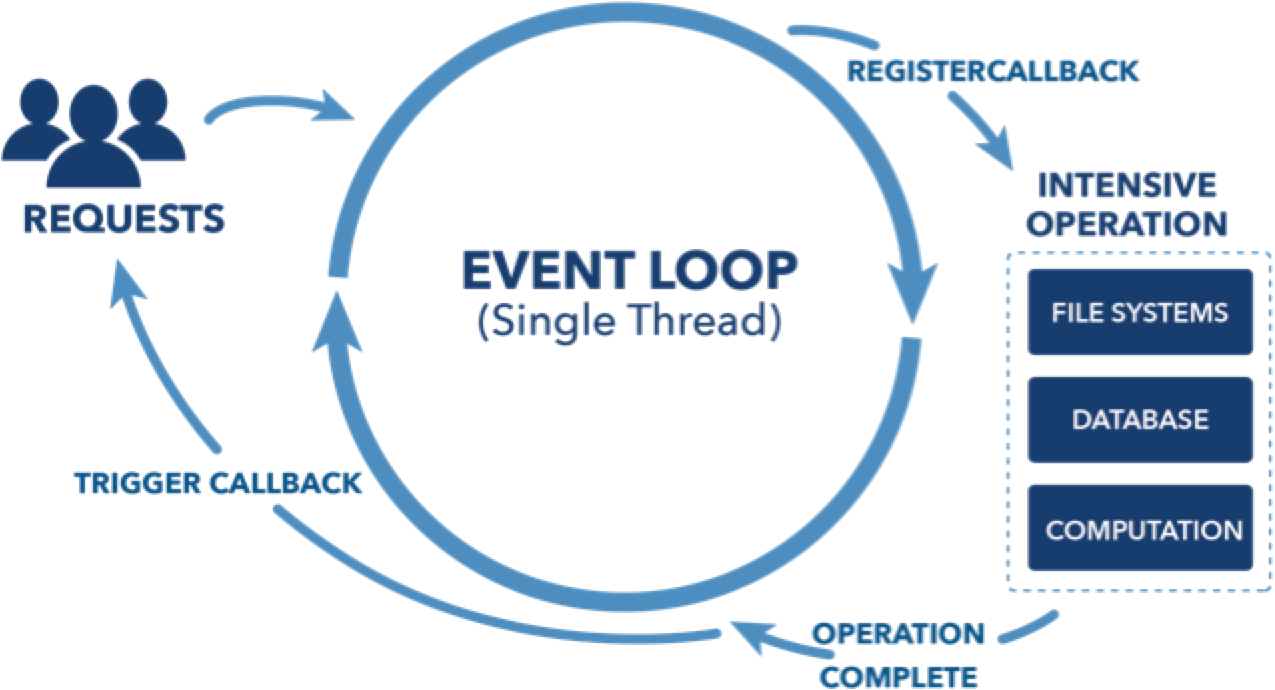
\includegraphics[width=\textwidth]{images/nodeEvent.png}
	\caption{Gestione eventi con Node.js.}
	\label{fig:nodeEvent}
\end{figure}
Bisogna però sempre tenere a mente, quando si progetta di scrivere un programma con Node.js, che questa architettura ha un effetto collaterale molto pesante; le operazioni che occupano per lungo tempo il thread in cui viene eseguito il codice (operazioni di calcolo onerose) bloccano l'interno software. Per questo motivo Node.js è assolutamente sconsigliato in caso di operazioni di calcolo complesse e nella fase di progettazione di programmi che usano questa piattaforma è sempre necessario utilizzare questa caratteristica come criterio fondamentale per la scrittura del codice.
Di seguito sono alcune delle caratteristiche importanti che rendono Node.js la prima scelta di architetti del software:
\begin{itemize}
\item \textbf{Asynchronous and Event Driven}: Tutte le API della libreria Node.js sono asincrone, ovvero non bloccanti. Significa essenzialmente che un server basato su Node non aspetta mai che un'API restituisca i dati. Il server passa all'API successiva dopo averlo chiamato ed un meccanismo di notifica di eventi consente al server di ottenere una risposta dalla precedente chiamata.
\item \textbf{Molto veloce}: Essendo costruito sul motore Javascript V8 di Google Chrome, Node.js è molto veloce nell'esecuzione del codice.
\item \textbf{Thread singolo ma altamente scalabile}: Node utilizza un singolo thread con loop di eventi. Il meccanismo degli eventi aiuta il server a rispondere in modo non bloccante e rende il server altamente scalabile rispetto ai server tradizionali che creano thread limitati per gestire le richieste. Quindi, Node utilizza un singolo programma con thread e lo stesso programma può fornire il servizio a un numero molto più grande di richieste rispetto ai server come Apache HTTP Server.
\item \textbf{Nessun Buffering}: Le applicazioni create con node non bufferizzano mai alcun dato. Queste applicazioni generano semplicemente i dati in blocchi.
\item \textbf{Licenza}: Node è rilasciato sotto licenza MIT. 
\end{itemize}
Esiste un mondo attorno a Javascript composto da librerie che ne estendono le funzionalità. Stesso discorso vale per Node.js, in quanto è attiva una comunità di sviluppo che ha realizzato in questi anni molte librerie per realizzare particolari tipi di supporto (database, Network, . . . ) ed un sistema di installazione di questi moduli che si occupa anche di eventuali dipendenze: \textit{npm}. Nei prossimi capitoli saranno analizzati alcuni progetti legati a Node.js usati nella creazione della webapp.

\subsubsection{Express.js ed Handlebars}
\label{sec:express handlebars}
Express.js (anche chiamato semplicemente Express) è un framework basato su Node.js che offre un insieme robusto di utilità per realizzare agilmente un'architettura \textit{MVC (Model-View-Controller)} sul lato server di applicazioni web single-page, multi-page ed ibride.
\\Basato sul modulo di Node chiamato \textit{connect}, risulta essere un ottimo "connettore" o \textit{middleware} tra le diverse librerie che possono popolare una webapp, tra cui WebSocket, Passport, Mustache.js, Handlebars, etc.
\\Le funzionalità offerte sono il \textit{routing}, la possibilità di gestire le configurazioni dell'applicazione ed un motore di templating.
\\Al centro di questa libreria c'è il concetto di flusso di funzioni, o come piace dire a certe persone, un set di \textit{livelli di funzione}. Infatti, per creare un'applicazione Express c'è bisogno di creare una sequenza di funzioni (livelli) che il framework può navigare. 
\\Quando una di queste decide di entrare in gioco, può completare il processo e fermare la sequenza. Dopodiché Express riprende a scorrere la sequenza fino alla fine.
\\Queste funzioni hanno delle callback associate che sono eseguite nel momento in cui un client effettua una richiesta. Questo processo prende il nome di Routing.
\\Il routing, dunque, è una funzionalità di Express.js, che determina la risposta ad una richiesta client ad un endpoint particolare; il quale può essere un URI (o percorso) o un metodo di richiesta HTTP specifico. In pratica, con Express, si possono gestire le richieste e le risposte \textit{in the middle}, cioè fra server e client. Quando il server riceve una richiesta HTTP la racchiude all'interno di un oggetto \textit{ServerRequest}. Questo oggetto, insieme all'oggetto \textit{ServerResponse}, viene passato al primo middleware che ne può modificare il contenuto, o aggiungere proprietà. Una volta terminata la modifica, il middleware richiamerà il successivo nell'eventuale catena (di funzioni) presente.
\begin{figure}[H]
	\centering
	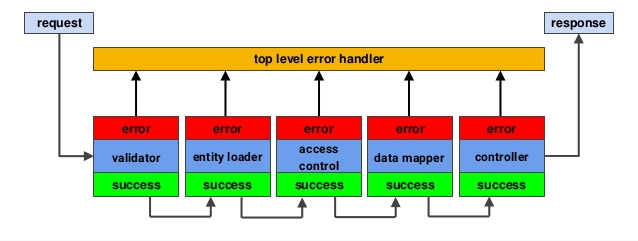
\includegraphics[width=\textwidth]{images/ExpressRoute.png}
	\caption{Visualizzazione della catena di funzioni per rispondere ad una richiesta}
	\label{fig:expressFlow}
\end{figure}
Se l'ultima funzione della catena deve restituire un HTML come risultato, Express chiama in causa il \textit{template engine}. Questo motore, infatti si occupa di fare il tramite tra i dati presenti nel layer model e quello di presentazione. In particolare elabora la richiesta producendo, in fase di run-time, un HTML dinamico partendo da una struttura definita (template). Esistono diversi motori che possono essere utilizzati con Express ognuno con le proprie particolarità e specifiche. 
\\Per questo elaborato la scelta del templating engine è caduta su \textit{Handlebars.js}. La libreria di templating Handlebars consente di creare un'interfaccia utente ricca includendo HTML statico e contenuto dinamico, che possono essere specificati nelle doppie parentesi graffe. Handlebars.js è molto popolare, semplice da usare e con una grande community. È basato sul linguaggio dei modelli di Mustache, ma lo migliora in molti aspetti. Con Handlebars, si può separare la generazione di HTML dal resto del JavaScript e scrivere codice più pulito. Inoltre, aggiunge costrutti (if e cicli for) che permettono di creare dinamicamente l'HTML. Infine, introduce un sistema di \textit{partial} che permette allo sviluppatore di inserire nelle proprie pagine, porzioni di HTML provenienti da file esterni. 
\\Express, quindi, per costruire la pagina di risposta da inviare al client, chiama Handlerbars che preleva i file con estensione \textit{.handlebars} li "compila" e genera il risultato finale.

\begin{lstlisting}[language=HTML, label=lst:HandlebarsTemplate, caption={Esempio di HTML scritto con Handlebars.}]
<div class="entry">
  <h1>{{title}}</h1>
  <h2>By {{author.name}}</h2>
  <div class="body">
    {{body}}
  </div>
</div>
\end{lstlisting} 

Il listato \ref{lst:HandlebarsTemplate} è un esempio di HTML scritto con la sintassi di Hadelbars. I valori \textit{title}, \textit{author.name} e \textit{body} saranno sostituiti, in fase di run-time, con i valori provenienti dal controller che passerà un oggetto all'engine templating. vedi listato \ref{lst:handleCode}.

\begin{lstlisting}[language=Javascript, label=lst:handleCode, caption={Esempio di variabile passata dal controller al template engine.}]
var context = {
  title: "My First Blog Post!",
  author: {
    id: 47,
    name: "Yehuda Katz"
  },
  body: "My first post. Wheeeee!"
};
\end{lstlisting} 

\subsubsection{WebSocket}
\label{sec:WebSocket}
L'applicazione web dell'elaborato di tesi, come detto in precedenza, prevede una interfaccia grafica per la visualizzazione delle ultime transazioni provenienti da Bitcoin. Per poter implementare questa funzionalità, c'è bisogno di utilizzare tecniche che permettano l'invio di dati tra client e server. Dal semplice request/response di HTTP, l'evoluzione del web e delle sue tecnologie ha portato alla nascita di nuove tecnologie per migliorare sempre di più la comunicazione remota.
\\Il modello tradizionale di comunicazione, derivato dalle specifiche standard di HTTP, prevedeva una comunicazione sincrona: in seguito a una azione dell'utente (request), il server eseguiva l'operazione richiesta e restituiva il risultato (response). Dopo la richiesta iniziale, il client si poneva in uno stato di attesa fino a quando la risposta non era ricevuta, risultando in uno spreco di tempo e risorse. Il refresh della pagina peggiorava inoltre la user-experience. Allo stesso tempo, il server non manteneva nessuna informazione riguardo alla comunicazione appena avvenuta. Più richieste della stessa operazione dunque venivano ogni volta re-processate e rigenerate per ogni client che le richiedeva. Una comunicazione di questo tipo, semplice da effettuare dal punto di vista implementativo, risulta tuttavia inefficiente e inadatta ad applicazioni di larga scala moderne.
\\Il primo fondamentale passo è stato rendere la comunicazione da sincrona ad asincrona. Ciò è stato possibile attraverso l'uso di plugin esterni, come Flash, oppure tramite nuovi meccanismi come Ajax. Tuttavia, entrambi presentano dei problemi: nel primo caso, un utente poteva non aver intenzione di installare software esterno, rendendo così inutile il plugin; nel secondo caso, la gestione stessa della comunicazione attraverso Javascript poteva velocemente raggiungere livelli di complessità non accettabili per grandi applicazioni. Per questi motivi la comunicazione tra client e server distribuito, è implementata con l'utilizzo della nuova tecnologia associata ad HTML5: i \textit{WebSocket}.
Formalmente, WebSocket è una tecnologia web che fornisce canali di comunicazione full-duplex attraverso una singola connessione TCP. L'API del WebSocket è stata standardizzata dal W3C e il protocollo WebSocket è stato standardizzato dall'IETF come RFC 6455 \cite{websocket:wiki}.
\\Dunque, tra le novità portate da HTML5, i WebSocket rappresentano quella di maggior importanza dal punto di vista dell'interazione tra client e server. WebSocket è una tecnologia per effettuare comunicazioni bidirezionali in tempo reale. Essi prevedono un canale di comunicazione sempre attivo, a bassa latenza, tra client e server, utilizzabile da entrambi sia in scrittura che in lettura. Tale canale è costituito da una connessione TCP persistente, garantito da un handshaking client-key iniziale ed un modello di sicurezza originbased. Per la protezione dei dati trasmessi contro lo sniffing sono applicate apposite maschere. 
\\Le caratteristiche principali dei WebSocket:
\begin{itemize}
\item \textbf{Bidirezionali}: Quando il canale di comunicazione è attivo, sia il client che il server sono connessi ed entrambi possono inviare e ricevere messaggi.
\item \textbf{Full-duplex}: Dati inviati contemporaneamente dai due attori (client e server) non generano collisioni e vengono ricevuti correttamente.
\item \textbf{Basati su TCP}: Il protocollo usato a livello di rete per la comunicazione è il TCP, che garantisce un meccanismo affidabile (controllo degli errori, re-invio di pacchetti persi, ecc) per il trasporto di byte da una sorgente a una destinazione.
\item \textbf{Client-key handshake}: All'apertura di una connessione, il client invia al server una chiave segreta di 16 byte codificata con base64. Il server aggiunge a questa un'altra stringa, detta \textit{magic string}, specificata nel protocollo (“258EAFA5-E914-47DA-95CA-C5AB0DC85B11”), codifica con SHA1 e invia il risultato al client. Cosi facendo, il client può verificare che l’identità del server che ha risposto corrisponda a quella desiderata.
\item \textbf{Sicurezza origin-based}: Alla richiesta di una nuova connessione, il server può identificare l'origine della richiesta come non autorizzata o non attendibile e rifiutarla.
\item \textbf{Maschera dei dati}: Nella trama iniziale di ogni messaggio, il client invia una maschera di 4 byte per l'offuscamento. Effettuando uno XOR bit a bit tra i dati trasmessi e la chiave è possibile ottenere il messaggio originale. Ciò è utile per evitare lo sniffing, cioè l'intercettazione di informazioni da parte di terze parti.
\end{itemize}
\begin{figure}[H]
	\centering
	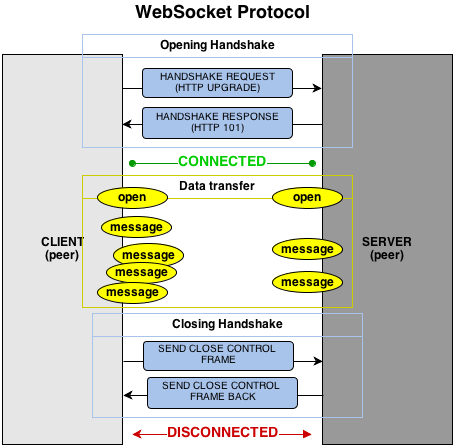
\includegraphics[width=\textwidth]{images/websocketProtocol.png}
	\caption{Comunicazione client/server tramite WebSocket}
	\label{fig:websocketProtocol}
\end{figure}
WebSocket è disegnato per essere implementato sia lato browser che lato server, ma può essere utilizzato anche da qualsiasi applicazione client-server. L'utilizzo dei WebSocket lato client, è possibile attraverso l'uso di specifiche API Javascript che consentono di ottenere informazioni sullo stato della connessione (aperta, chiusa, in apertura o in chiusura), di interagire con essa (inviare dati o chiudere la comunicazione) o di gestire particolari eventi come la ricezione di errori. Lato server, invece, esistono implementazioni dei WebSocket per la maggior parte dei linguaggi più utilizzati (Node.js, Java, C\#, Python, Ruby).

\subsubsection{MaterializeCSS}
\label{sec:materialCSS}
L'interfaccia grafica, \textit{GUI (Graphical User Interface)} o \textit{UI (User Interface)}, di una applicazione web determina, in molti casi, il suo successo. Progettare e programmare bene questo componente, quindi, ha un peso molto importante sulla buona riuscita anche del sistema sottostante che lo alimenta. 
\\Materialize CSS è una libreria che permette di creare interfacce in \textit{Material Design}. Creato e progettato da Google, Material Design è un linguaggio di progettazione che combina i principi classici del design di successo con l'innovazione e la tecnologia. L'obiettivo di Google è sviluppare un sistema di progettazione che consenta un'esperienza utente unificata su tutti i loro prodotti. Sebbene si possa scegliere tra milioni di librerie, la scelta di questo tool risulta molto promettente ed è una valida alternativa a prodotti affermati, quali Bootstrap o Foundation, con i quali è molto più complicato produrre un'interfaccia con una vera identità. MaterializeCSS dunque è un framework CSS usato per creare siti \textit{responsive}. Offre layout, animazioni e molti altri componenti che rendono semplice la creazione di pagine web.
\\Le principali caratteristiche sono:
\begin{itemize}
\item \textbf{Installazione}: L'installazione del framework è estremamente semplice, infatti bisogna solo importare i CSS e i javascript nel tag head nelle pagine html del proprio sito.
\item \textbf{Grid System}: Materialize divide il layout di un pagina web in 12 colonne. Questo sistema prende il nome di \textit{grid system} e permette di utilizzare classi \textit{container} che rendono il sito responsive e quindi utilizzabile su ogni dispositivo.
\item \textbf{Componenti}: Il framework ha una moltitudine di componenti \textit{pronti all'uso}. E' possibile   
\end{itemize} 

\subsubsection{D3.js}
\label{sec:d3js}
Ultimo componente di maggiore interesse è la libreria \textit{D3.js}. Questa libreria è usata all'interno di MaterilizeCSS per disegnare i grafi delle transazioni. D3.js (o solo D3 per Data-Driven Documents) è una libreria Javascript scritta da Mike Bostock come progetto successore di un precedente tool di visualizzazione chiamato Protovis. E’ basata sugli standard web e sfrutta appieno le tecnologie dei browser per manipolare gli elementi: come per JQuery, si utilizza la sintassi CSS per i selettori e si applicano gli stili agli elementi tramite fogli CSS. D3 a differenza delle altre librerie di grafici, non offre un insieme di grafici già pronti all'uso, bensì un potente framework che permette di realizzare praticamente qualsiasi tipo di grafico manipolando gli elementi di una pagina web di tipo HTML, SVG o Canvas in base al contenuto di un dataset.
\\La libreria JavaScript D3, incorporata in una pagina web HTML, utilizza funzioni JavaScript prefatte per selezionare elementi del DOM, creare elementi SVG, aggiungergli uno stile grafico, oppure transizioni, effetti di movimento e/o tooltip. Questi oggetti posso essere largamente personalizzati utilizzando lo standard web dei "fogli di stile a cascata", chiamati in inglese CSS. In questo modo grandi collezioni di dati possono essere facilmente convertiti in oggetti SVG usando semplici funzioni di D3 e così generare ricche rappresentazioni grafiche di numeri, testi, mappe e diagrammi. I dati utilizzati possono essere in diversi formati, il più comune è il JSON, valori separati da virgola CSV o geoJSON, ma, se necessario, di possono scrivere funzioni JavaScript apposta per leggere dati in altri formati. Il concetto centrale del design di D3 è permettere al programmatore di usare dei selettori, come per i CSS, per scegliere i nodi all'interno del DOM Document Object Model e quindi usare operatori per manipolarli, similmente alla libreria jQuery (see Bostock, Ogievetsky e Heer, chap. 3). La selezione può essere basata su tag (come nell'esempio qui sopra), elementi, classi, identificatori, attributi o punti della gerarchia. Una volta che gli elementi sono selezionati possiamo applicare operazioni su di essi. Questo comprende leggere ed impostare attributi, mostrare testi, formattare. Gli elementi possono anche essere aggiunti e rimossi. Questo processo di modifica, creazione ed eliminazione di elementi HTML, può essere eseguito in base ai set di dati forniti, che è il concetto di base di D3.js.